The implementation of LM is composed of a compiler and a virtual machine~(VM).
Figure~\ref{fig:implementation:overview} presents an overview of the compilation
process for LM programs. The two main boxes represent the two major components
of the system, namely, the compiler and virtual machine.

\begin{figure}
  \centering
  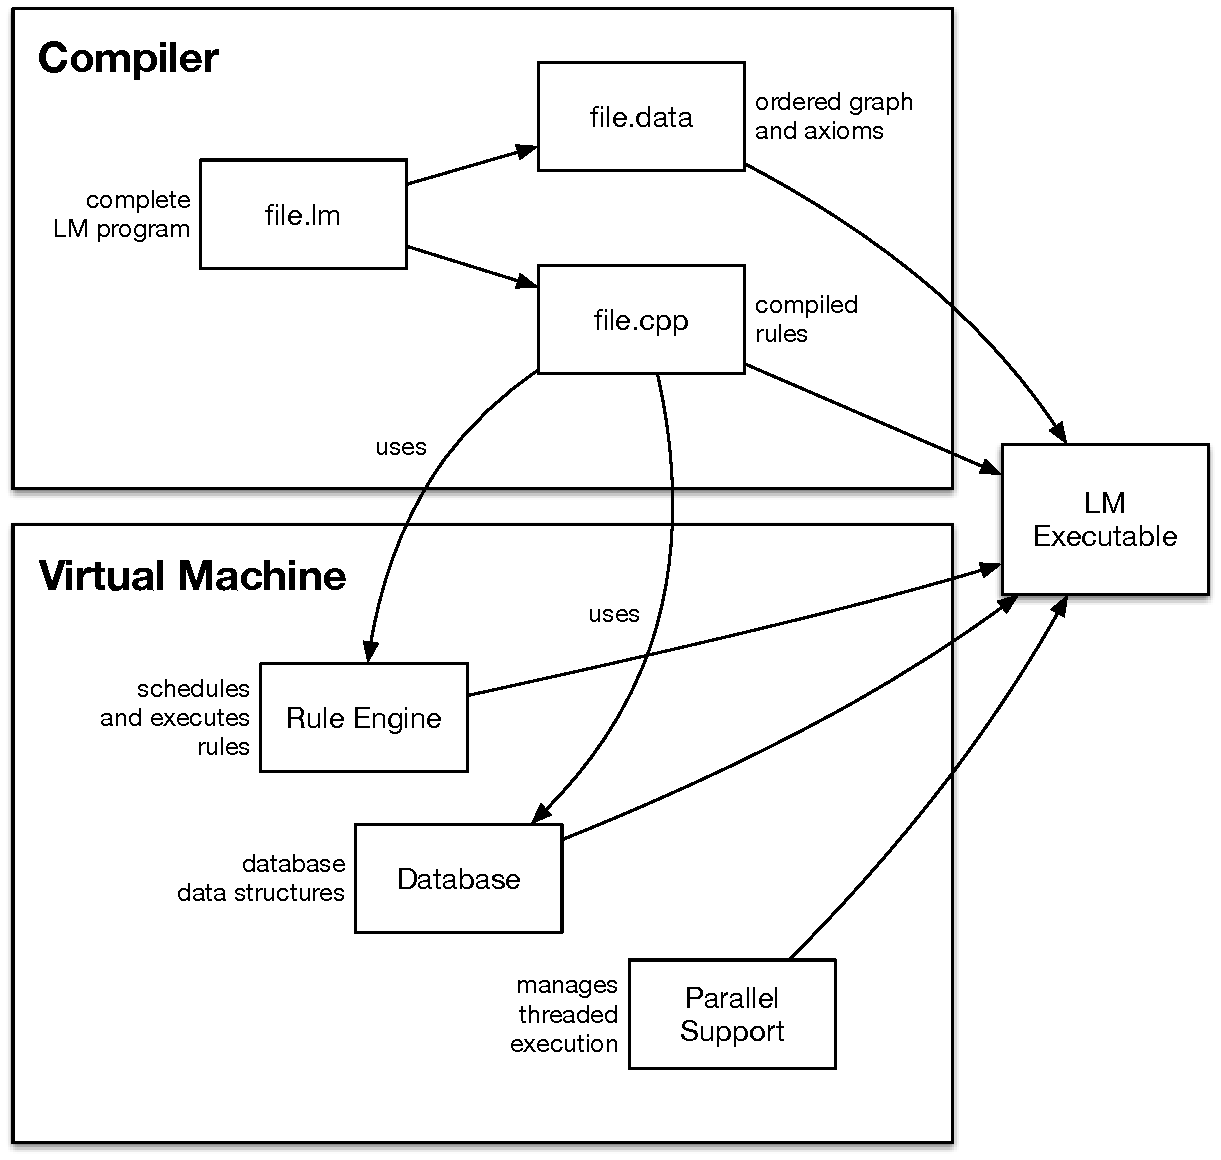
\includegraphics[width=.8\linewidth]{figures/implementation/overview.pdf}
  \caption{Compilation of a LM program into an executable. The compiler
     transforms a LM program into \texttt{file.cpp}, C++ file with compiled
     rules, and a \texttt{data} file with the graph structure and axioms. The virtual
     machine which includes code for managing multithreaded execution and the
     database of facts is then linked with \texttt{file.cpp} to create a
     standalone executable that can be run in parallel.}
  \label{fig:implementation:overview}
\end{figure}

The virtual machine contains supporting data structures for managing the
database of facts and to schedule the execution of rules. The parallel engine is
also a major part of the virtual machine and is responsible for managing
multithreaded execution by launching threads, managing communication and
and scheduling parallel execution, including coordination.

The compiler transforms LM files into C++ code that use the virtual machine
facilities to implement the program logic.  The compiled code implements the
inference rules of the program and uses the API of the virtual machine to derive
and retract facts and to schedule the execution of rules.  The compiler also
creates a separate file, named \texttt{file.data}, with the program's axioms and
graph structure. The graph structure is reconstructed in parallel once the
program starts.

To complete the compilation process, we use a C++ compiler to compile the
virtual machine files and \texttt{file.cpp} into object files that are then
linked along with \texttt{file.data}. At the end, we have a standalone
executable that allows the user to input the number of threads to use,
scheduling strategies (i.e., disable coordination), run time measurement
facilities and also database printing facilities.

Alternatively, the programmer may also decide to compile a more general version
of the virtual machine that is able to run byte-code files generated by the
compiler. This allows faster development since the programmer only needs to
recompile the LM program and not the whole stack. However, LM programs will run
slower since the byte-code must be interpreted by the virtual machine. This
severely affects programs with many mathematical operations, especially floating
point computations.

\subsection{Graph Clustering}

The graph structure stored in file \texttt{file.data} is constructed by the
compiler by analyzing the program's axioms and then ordering the nodes of the
graph.  In order to distribute computation across threads it is important to
increase locality of communication, so that a node makes most of its
communication to neighbor nodes that are being handled by the same thread. The
graph structure in \texttt{file.data} is written in order to improve locality
and reduce communication between threads.

The compiler analyzes the node address constants (that are prepended by the
symbol @) and the axioms of the program. After parsing and type-checking the
program code, the compiler then optimizes the topology by building an internal
representation of the graph.  In this phase, each node address $a$ is mapped
using a function $M(x)$ to a normalized node address $n$. Function $M(x)$ is
bijective and the domain is the set of all nodes described in the source code.
The codomain of $M$ is the discrete interval $[0, N[$, where $N$ is the number
of nodes in the graph. The byte-code of a LM program includes all the pairs $(x,
M(x))$ so that the runtime system can put this information to use.

We have three methods for defining the function $M(x)$:

\begin{itemize}
   \item \emph{Static}: the compiler uses the node addresses presented in the
      code as long as they fill the discrete interval $[0, N[$.
   \item \emph{Randomized}: the mapping is done randomly.
   \item \emph{Breadth-First}: the mapping is built by picking an arbitrary node, $n_{zero}$
   and setting $M(n_{zero}) = 0$, then we select all neighbors of $n_{zero}$ and start defining
   their mappings in increasing order, $1, \dotsc, N-1$, and adding its neighbors for later processing
   in a breadth first fashion.
\end{itemize}

The breadth-first method is used with the intent of clustering closer nodes in
an ordered fashion.  While not optimal, using a breadth-first approach is very
efficient and has good results for irregular graphs. If we use a static division
of work between $N$ threads, where each thread is responsible to process a
pre-defined set of nodes, we can efficiently slice the codomain of function
$M(x)$ and divide it between the $N$ threads.

For an example, consider the graph in Fig.~\ref{fig:compiler:topology1}. The
node addresses represented are the ones included in the source code. Using a
breadth-first method starting by node 1, we get the following order: 1, 2, 3, 7,
5, 6 and 4. If we had to do a static division with 2 threads, thread 1 would get
1, 2, 3, 7 and thread 2 would get 5, 6 and 4. Note from
Fig.~\ref{fig:compiler:topology1} that only 3 edges exist between the nodes of
thread 1 and thread 2. This greatly reduces communication between threads and
improves parallel efficiency.

\begin{figure}[ht]
  \centering
  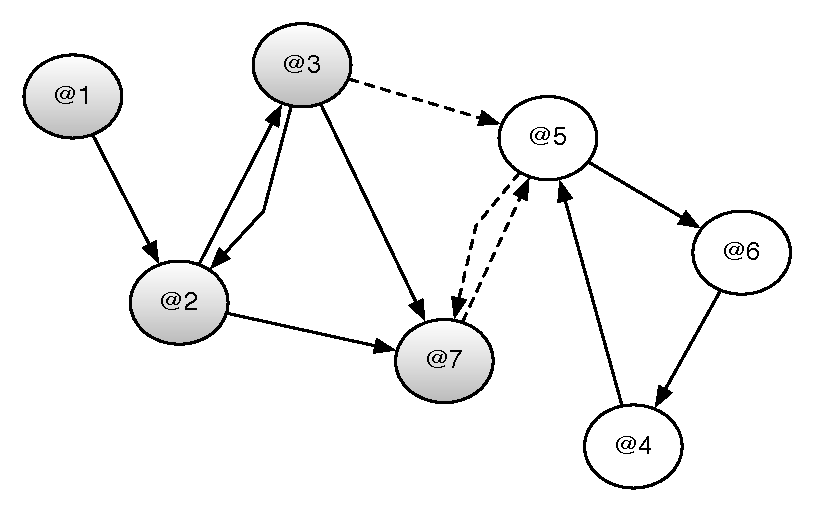
\includegraphics[width=0.6\textwidth]{figures/compiler/topology1.pdf}
  \caption{Topology using a breadth-first method.}
  \label{fig:compiler:topology1}
\end{figure}
